\documentclass[a4paper]{article}

\usepackage[utf8]{inputenc}
\usepackage{erk}
\usepackage{times}
\usepackage{graphicx}
\usepackage[top=22.5mm, bottom=22.5mm, left=22.5mm, right=22.5mm]{geometry}

\usepackage[slovene,english]{babel}
\usepackage{hyperref}
\usepackage{url}

\let\oldfootnotesize\footnotesize
\renewcommand*{\footnotesize}{\oldfootnotesize\scriptsize}

\begin{document}
\title{POROČILO IZDELAVE IGRE - AIRBORNE \\
 Računalniška grafika in tehnologija iger, FRI 2022}

\author{Luka Uranič$^{1} (63200035)$, Alen Kurtagić$^{1} (04200012)$,  Ana Maurič$^{1} (64190013)$, \\ Anja Jerala$^{2}$,  Nika Črne$^{2}$} % use ^1, ^2 for author(s) from different institutions

\affiliation{	$^{1}$Univerza v Ljubljani, Fakulteta za računalništvo in informatiko \\ 
				$^{2}$Univerza v Ljubljani, Naravoslovnotehniška fakuteta}

%\email{E-pošta: ciril.bohak@fri.uni-lj.si}

\maketitle

\selectlanguage{slovene}

\begin{abstract}{Abstract}%done
Airborne je letalska igra, narejena v WebGL-ju. Idejo za igro je v tej skupini podal Alen, navdušila ga je letalska tekmovalna igra Air Wars 3 in podobni seminarji pri RGTI-ju iz prejšnjih let. Ker nam je bila ideja drugim članom všeč, smo jo uporabili, razvili in nadgradili v končni izdelek. Ko smo se združili še z oblikovalkama iz NTF-ja, smo idejo tudi malce spremenili glede na njune želje in predloge. Želeli smo ustvariti interaktvino, zanimivo igro, ki bi igralca pritegnila z napetim dogajanjem, realistično sceno in pa tudi lepo vizualno podobo. Delo je bilo razdeljeno na dva osnovna dela: oblikovanje in izvoz modelov (letala in ostalih modelov sveta) v Blenderju ter potem programiranje igre v WebGL-ju. Pomagali smo si z materialom iz vaj in tutoriali na Youtube-u od kreatorja Andrew-a Adamsona \footnote{\url{https://www.youtube.com/playlist?list=PLPbmjY2NVO_X1U1JzLxLDdRn4NmtxyQQo}}. Celotno delo je trajalo približno 1 mesec. 
\begin{center}
     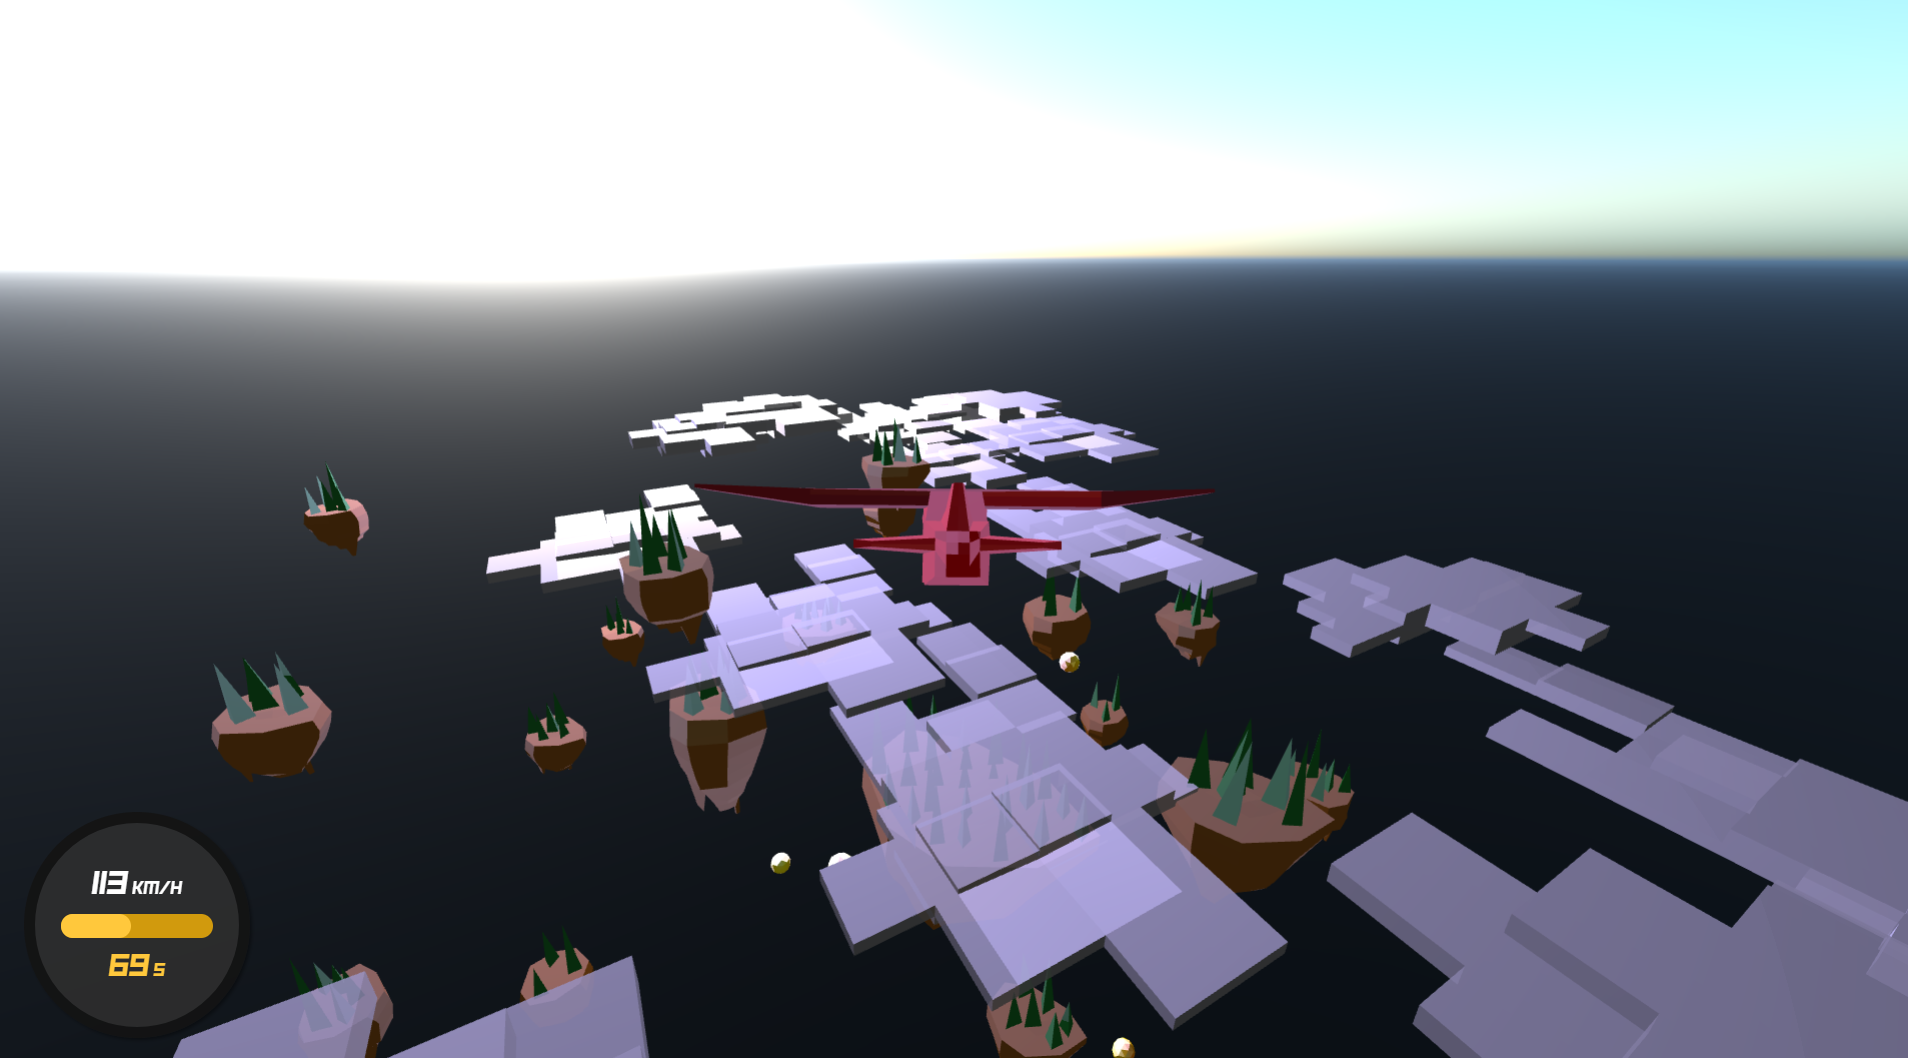
\includegraphics[width=\columnwidth]{igra.jpg}
\end{center}
\end{abstract}

\section{Pregled igre}%done
Igra Airborne je letalska igra iz perspektive 3. osebe. Igralec oz. pilot usmerja letalo, s katerim poskuša nabrati žetone, ki mu povečujejo količino goriva. Igre je konec, ko se letalo zaleti v ovire v svetu ali pa ko mu zmanjka goriva. Igralec mora biti dovolj spreten, da se približa žetonom in jih pobere, brez da se zaleti v ovire, ki so postavljene blizu žetona, medtem ko letala ne more ustaviti, le usmerja po xyz osi sveta - zato je zahtevnost igre srednje zahtevnosti. Namenjena je vsem, ki si jo želijo igrati, tako izkušeni igralci kot tudi začetniki. Letalo se nahaja v zraku, okrog njega porazdeljeno po svetu so lebdeči otoki, oblaki in zlati žetoni, v ozadju je sončno obzorje. Cilj igre je preživeti oz. leteti čim dlje časa, pobrati čim več žetonov. Igralec lahko raziskuje svet po vseh smereh neba.

\subsection{Opis sveta}%done
Naš 3D svet je upodobljen s preprostimi (low-poly) 3D modeli, vendar je njegova podoba še zmeraj realistična. Rdeče letalo se vedno nahaja v sredini zaslona, svet se okoli njega razteza v vse tri xyz dimenzije. Letalo se lahko premika kamorkoli po teh smereh. Svet vsebuje še rjave lebdeče otoke, na katerih rastejo zelena drevesa, zlate žetone okoli teh otokov in bele oblake na nebu. V daljavi v neskončnosti se vidi sončno obzorje. Tla so črna.

\subsubsection{Pregled}%done
Glaven model v svetu je letalo. Letalo vidi iz 3. perspektive, nahaja se malo za njim, da ima pregled nad vsem okoljem pred in ob letalu. Igralec in letalo se ves čas igre nahajata na sredini zaslona. Z pilotiranjem letala se igralec potem obrača naokoli, se približuje in oddaljuje otokom, žetonom, oblakom in ozdaju. 

\subsubsection{Ozadje}%done
Ozadje sestoji iz neba in daljave. Igralec lahko zapusti območje lebdečih otokov in leti proti obzorju, ampak ga ne more doseči, ker se razteza v neskončnost in ker mu bo hitro zmanjkalo goriva. Za takšno ozadje smo se odločili, da se poskusimo vizualno čim bolj približati dejanskemu razgledu, ki ga vidijo piloti.

\subsubsection{Ključne lokacije}%done
Ključna lokacija v svetu je sredina, kjer se nahaja 10 lebdečih otokov. Samo na tej lokaciji lahko igralec najde žetone, za letalo predstavlja nahajališče dobrin, ostalo je samo ozadje - kot je podrobneje opisano v prejšnjem razdelku, to sta ne-interaktivno sončno obzorje in tla.

\subsubsection{Velikost}%done
Svet je velik, zajeta je pravzaprav cela atmosfera po kateri letijo realna letala. Razširja se v neskončnost levo, desno, naprej, nazaj, gor in dol. Na ta svet gledamo iz 3. perspektive, da si ga lahko v celoti ogledamo in obiščemo. 

\subsubsection{Objekti}%done
Vsi modeli, ki sestavljajo naš svet, so narejeni v Blenderju, v sami kodi pa so uporabljeni kot Gltf modeli. Naredila jih je članica oblikovalka Anja. Zasnovali smo jih kot preproste modele, da bi bil rendering igre še vedno kolikor toliko optimalen, ki pa so še vedno zanimivi na pogled. Ozadje pa sestavljajo objekti, v celoti narejeni v WebGL-u. Modeli so podrobneje predstavljeni v razdelku "Osebek", ostali objekti, ki pa zajemajo ozadje, pa v razdelku "Ozadje". 

\subsubsection{Čas}%done
Hitrost časa v našem svetu ni čisto enaka realenu času - letalo ima na voljo približno 20s, po izteku tega časa mu goriva zmanjka, če ne pobere nobenega žetona. V realen času bi to trajalo nekaj ur. Naše letalo je tudi malo počasnejše od realnih, doseže hitrost približno 150km/h.

\subsection{Igralni pogon in uporabljene tehnologije}%done
Uporabljene tehnologije za izdelavo igre so bile Blender in WebGL, za pogon poljubni spletni brskalnik, za deljenje kode pa Github platforma. Dodatnih ogrodij oz. orodij nismo potrebovali in nismo uporabljali.

\subsection{Pogled}%done
Kot že predstavljeno, je Airborne igra iz 3. perspektive. Odločili smo se za 3. namesto 1. perspektivo, ker smo želeli, da lahko igralec dejansko vidi naš model letala. Kamera je vezana na letalo, ker je to igralčev objekt premikanja. Vedno bo igralec pred seboj videl letalo in njegovo kolico. Kot gledanja je širok, da lahko še vedno vidi čim več okolice. Ko se letalo premika, se z njim premika tudi kamera.

\section{Osebek}%done
Glavni osebek oz. objekt igre je letalo. Nad njim ima igralec popoln nadzor v smislu premikanja (razen hitrosti). Preko njega igralec interaktira s ostalimi modeli in ozadjem. 
\begin{center}
     \includegraphics[width=\columnwidth]{letalo.jpg}
\end{center}

Lebdeči otoki so sestavljen objekt iz zemlje, drevesnih debel in krošenj. Nahajajo se v večjem številu na sredini sveta, okoli letala. Predstavljajo glavno oviro za letalo - če se zaleti v otok oz. v drevesa, ki rastejo na otoku, je igre konec. 
\begin{center}
     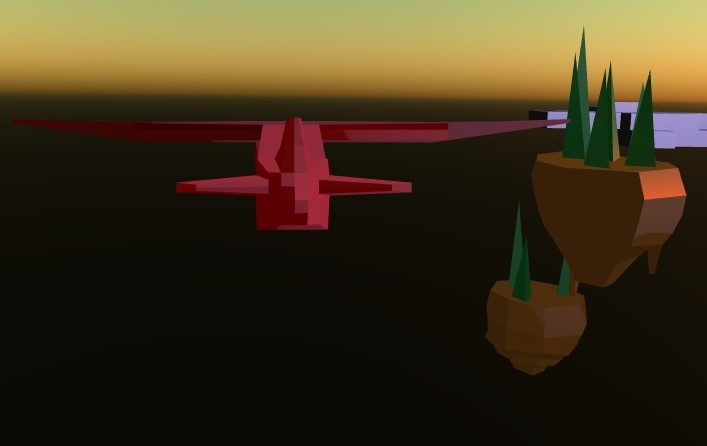
\includegraphics[width=\columnwidth]{Otoki1.jpg}
\end{center}

Žetoni so glavni objekt za interakcijo z letalo, so bistvo cele igre. Ko letalo pobere, torej se dotakne žetona, se mu poveča meter preostalega goriva.
\begin{center}
     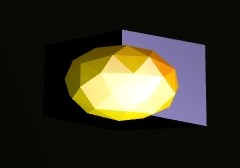
\includegraphics[width=\columnwidth]{zeton.jpg}
\end{center}

Preostanejo še oblaki, ki pa obstajajo le za realističen pridih. Niso ovire in hkrati letalu nič ne doprinesejo. Letalo lahko za zabavo leti skozi njih.
\begin{center}
     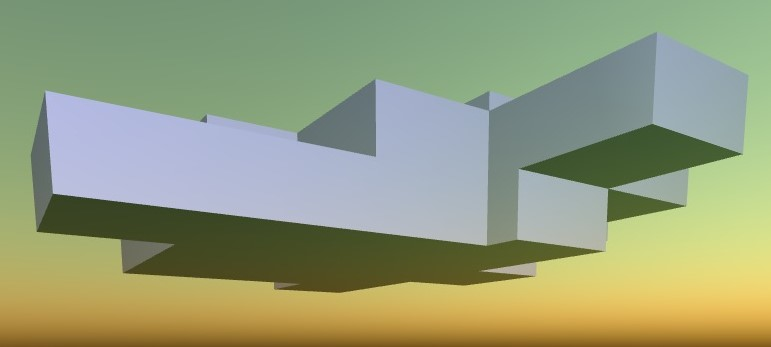
\includegraphics[width=\columnwidth]{Oblak.jpg}
\end{center}

Na otoke, oblake in žetone igralec nasploh ne more vplivati zunaj tega, da se v njih z letalom zaleti. 

\section{Uporabniški vmesnik}%done
Uporabnišli vmesnik za interakcijo je miška, miškina leva tipka in tipka ESC. Za to smo se odločili, ker miška omogoča gladko premikanje pogleda v vse smeri, kar vnese več realizma - nekako kot da zares pilotiramo letalo. Prav tako se v desnem zgornjem kotu nahaja uporabniški vmesnik z drsniki, s katerimi igralec nastavlja fizikalne lastnosti obzorja, da si lahko ozadje prilagodi po svojem okusu. V spodnjem levem kotu pa je še krog z informacijo, kako hitro leti letalo v km/h, meter, koliko goriva mu še preostane in pa čas v sekundah, ki jih preživi z letenjem.

\section{Glasba in zvok}%done
Za zvočne efekte uporabljamo zvok žvenketanja kovancev, ko letalo pobere žeton, in zvok zaleta, ko se letalo zaleti v oviro. Dodali smo ju za popestritev. Oba zvoka smo našli na internetu, sta royalty-free za takšno in podobno uporabo. \footnote{\url{https://www.link.si}}

\section{Gameplay}%done
Ko se igra zažene, se na zaslonu izpiše: "LEFT CLICK TO START". Takoj, ko igrale pritisne levo miškino tipko, se poveže z letalom in se začne premikati oz. leteti naprej. Igralec letala ne more ustaviti, z miškinim pogledom ga usmerja po xyz oseh. Če pritisne tipko ESC, se ta povezava prekine, na zaslonu se izpiše: "LEFT CLICK TO CONTINUE", kar da igro na pavzo, letala več ne nadzoruje in spet se lahko z miško premakne ven iz scene v brskalniku. Vsakič, ko pobere žeton, se zaigra zvok žvenketanja. Ko se zaleti, se predvaja zvok zaleta in ko mu zmanjka goriva, je igre konec, nima več nadzora nad letalom, izpiše se: "GAME OVER" in število sekund, ki jih je priigral. Zatem mora igro ponovno zagnati in začne na istem mestu, kot prej.
\begin{center}
     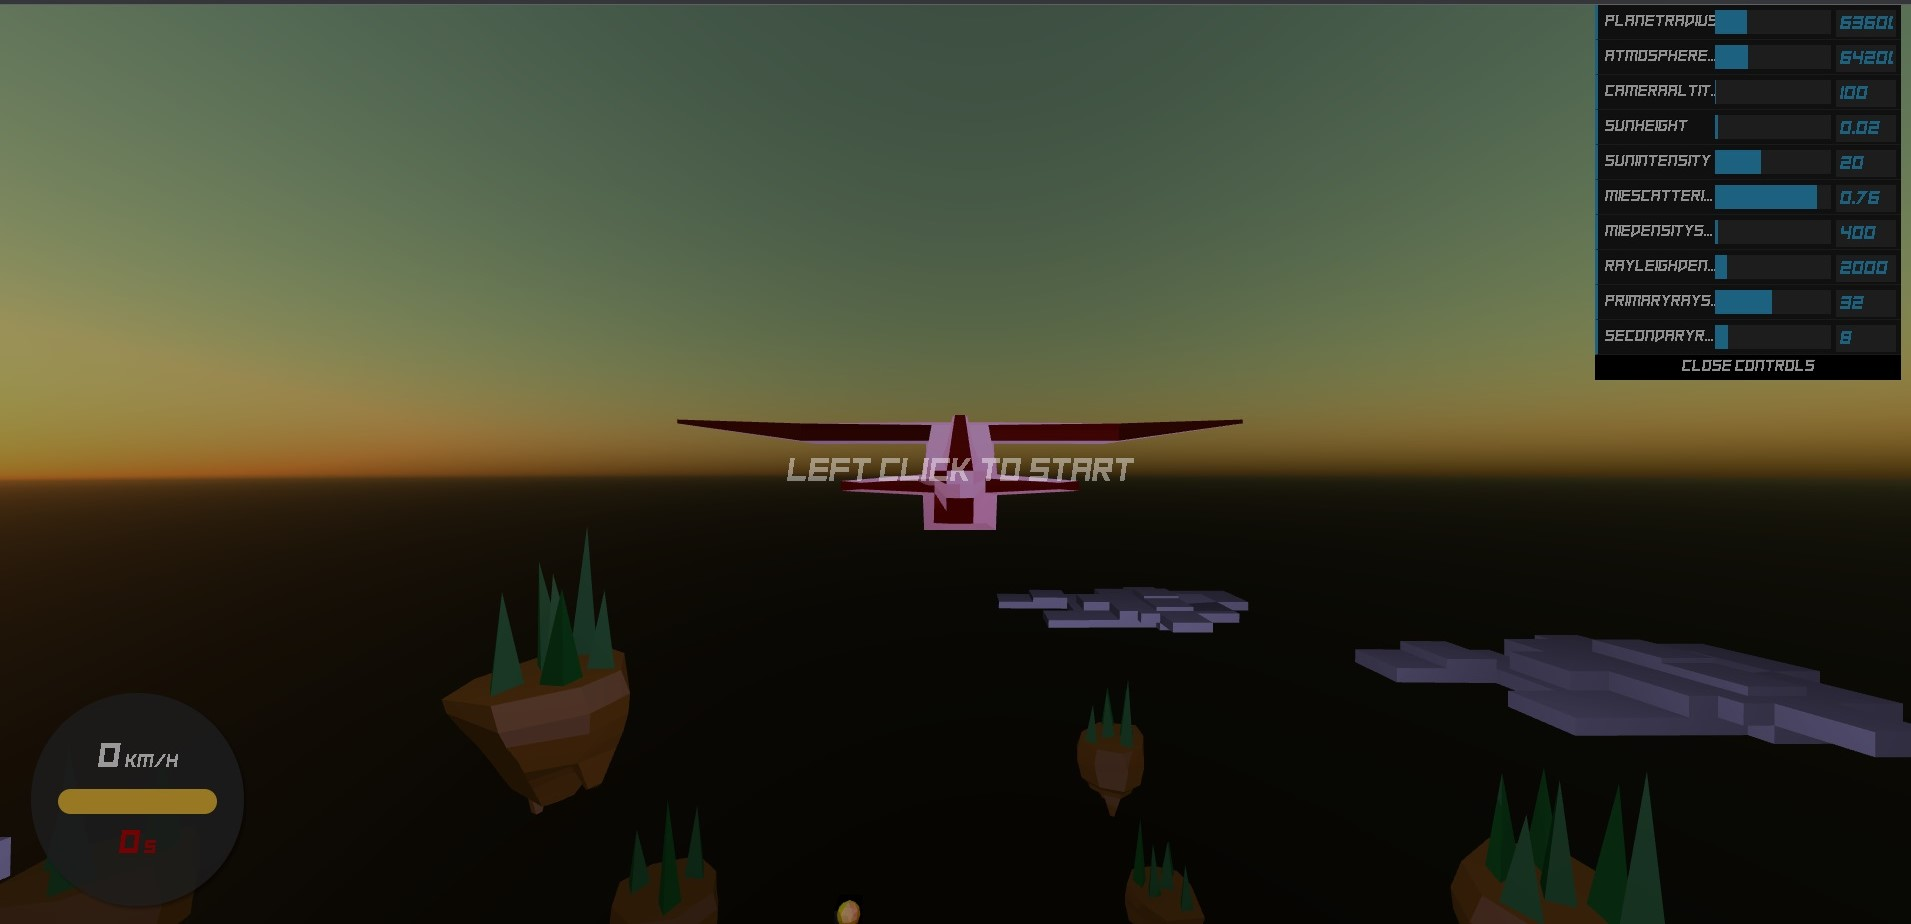
\includegraphics[width=\columnwidth]{start.jpg}
\end{center}

\begin{center}
     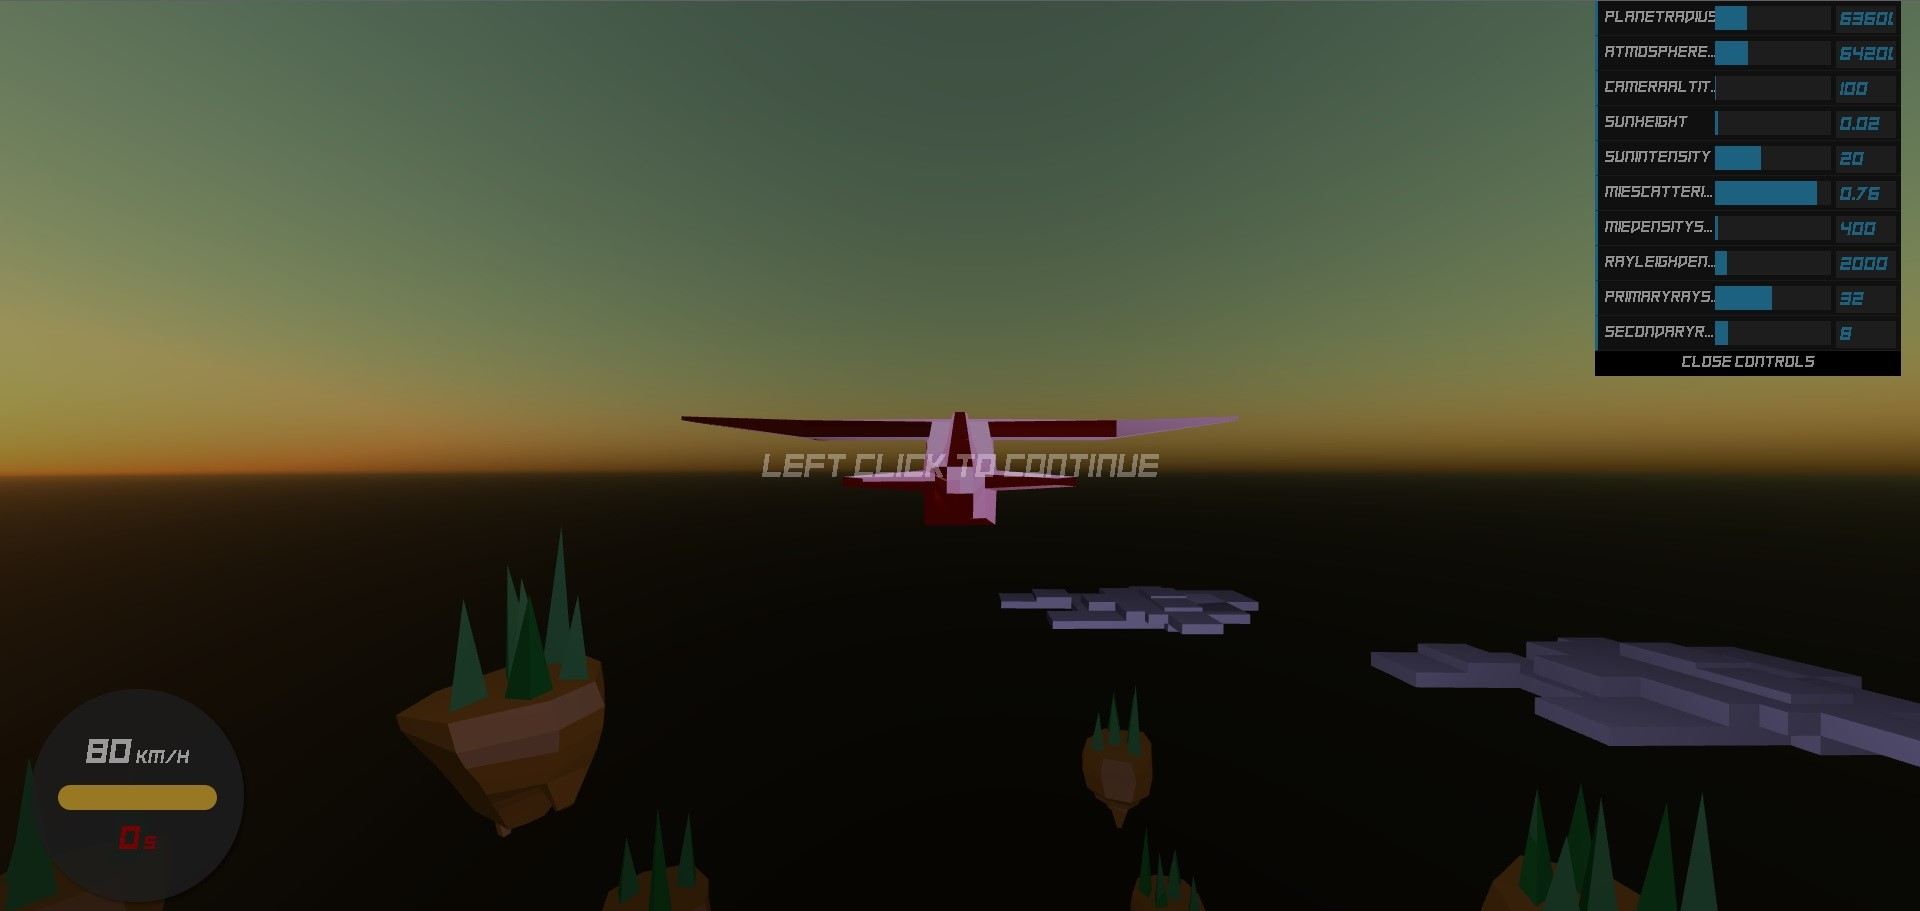
\includegraphics[width=\columnwidth]{continue.jpg}
\end{center}

\begin{center}
     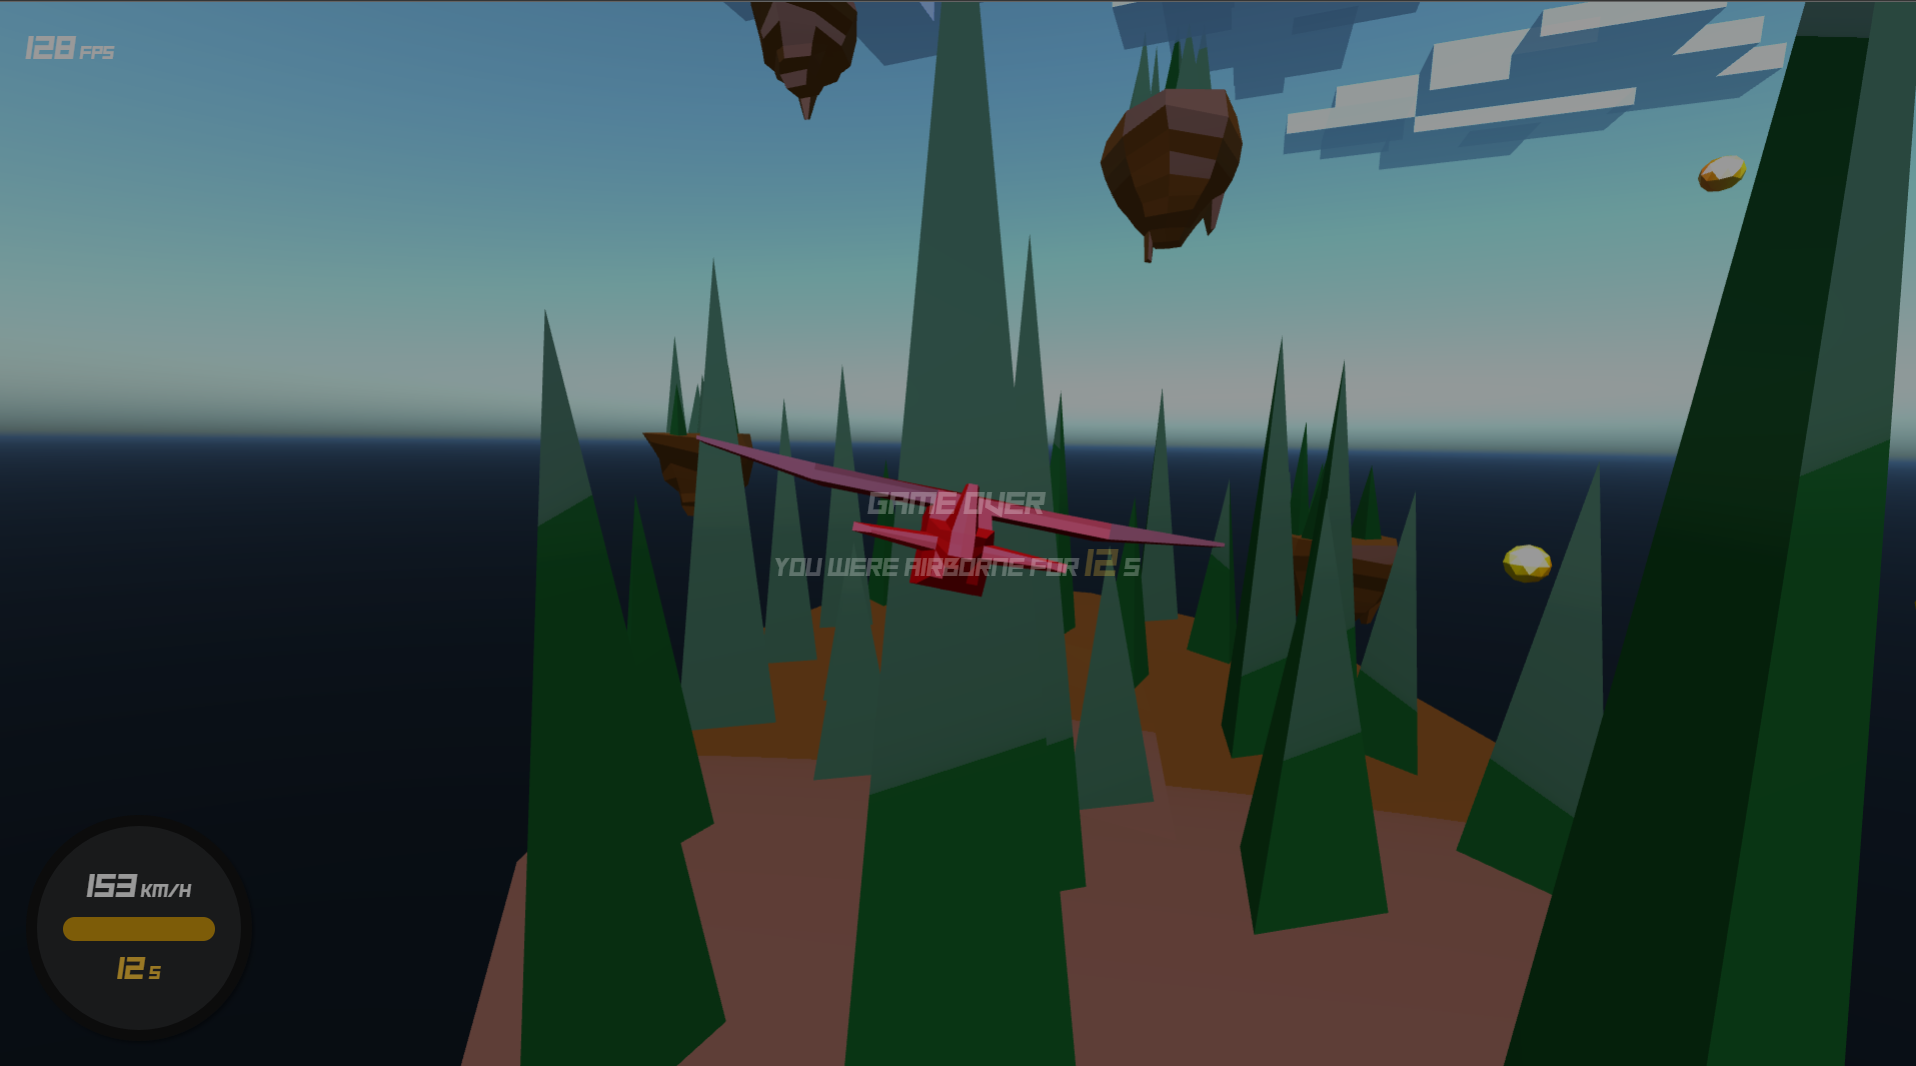
\includegraphics[width=\columnwidth]{game over.jpg}
\end{center}

\section{Tehnični vidiki igre} %done
\subsubsection{Izris prozornih objektov}%done
Pri izrisu prozornih objektov je pomembno, da jih izrišemo za neprozornimi objekti in urejene po bližini od kamere (najbližje najkasneje)

\section{Zaključki in možne nadgradnje} %done
Pri izdelavi smo v praksi utrdili teorijo iz predavanj, se naučili uporabe WebGL-a, nadgradili znanje JavaScripta in Githuba. Predviden scenarij smo uspeli izvesti v celoti, igra pa se v naslednjem projeku v Unityju lahko še nadgradi, doda več objektov, izboljša izgled in animacijo. Težave so se pojavljale pri kombiniranju logike oz. fizike sveta z gltf objekti. Koristilo bi, da bi na vajah naredili več primerov premikanja ipd. na dejanskih Gltf objektih, ne le na preprostih kockastih modelih.

\small
\bibliographystyle{plain}
%\bibliography{references}

\end{document}
